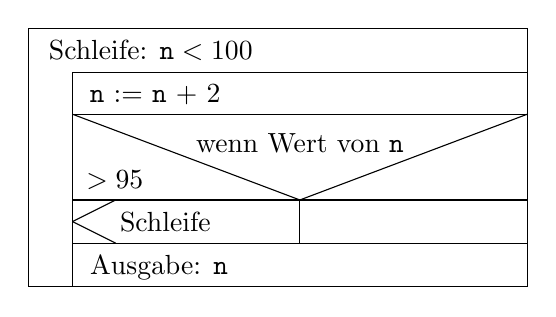
\begin{tikzpicture}
    \draw (0pt,0pt) rectangle (180.28222pt, -93.26682000000001pt);
    \node at (4.0pt, -46.633410000000005pt) {};
    \node at (44.28682pt, -8.01614pt) {Schleife: $\texttt{n} < 100$};
    \draw (16.03228pt,-16.03228pt) rectangle (180.28222pt, -31.08894pt);
    \node at (45.85599pt, -24.01686pt) {\texttt{n} := \texttt{n} + 2};
    \draw (16.03228pt,-31.08894pt) rectangle (180.28222pt, -62.0585pt);
    \node at (20.03228pt, -46.57372pt) {};
    \draw (16.03228pt, -31.08894pt) -- (98.15725pt, -62.0585pt);
    \draw (98.15725pt, -62.0585pt) -- (180.28222pt, -31.08894pt);
    \node at (31.28644pt, -54.74423pt) {$> 95$};
    \node at (176.28222pt, -58.0585pt) {};
    \node at (98.15724999999999pt, -41.412126666666666pt) {wenn Wert von \texttt{n}};
    \draw (16.03228pt,-62.0585pt) rectangle (98.15725pt, -77.66266pt);
    \node at (20.03228pt, -69.86058pt) {};
    \node at (49.58229pt, -69.86058pt) {Schleife};
    \draw (31.63644pt, -62.0585pt) -- (16.03228pt, -69.86058pt);
    \draw (16.03228pt, -69.86058pt) -- (31.63644pt, -77.66266pt);
    \draw (98.15725pt,-62.0585pt) rectangle (180.28222pt, -77.66266pt);
    \node at (102.15725pt, -69.86058pt) {};
    \draw (16.03228pt,-77.66266pt) rectangle (180.28222pt, -93.26682pt);
    \node at (47.270395pt, -86.529325pt) {Ausgabe: \texttt{n}};
\end{tikzpicture}
